\documentclass[../thesis.tex]{subfiles}
\begin{document}

\chapter{Molecular Lifetime Screening}\label{sec:hoye_solutionPL}
Design rules for stable emitters are not well developed, so it is possible that closely related molecules could have a significant change in stability.
A rapid screening technique is needed to brute force optimize emitter molecules for lifetime since the stability cannot be predicted a priori.
Ideally, this technique would probe the intrinsic stability of the emitter, rather than the stability of an OLED device, as device manufacturing requires optimization of its own.
The most isolated molecular properties can be probed in solution, where molecules are not in contact with each other.
Solution has the added advantage of easy processing, further enabling rapid screening.

\begin{figure}[ht]
\centering
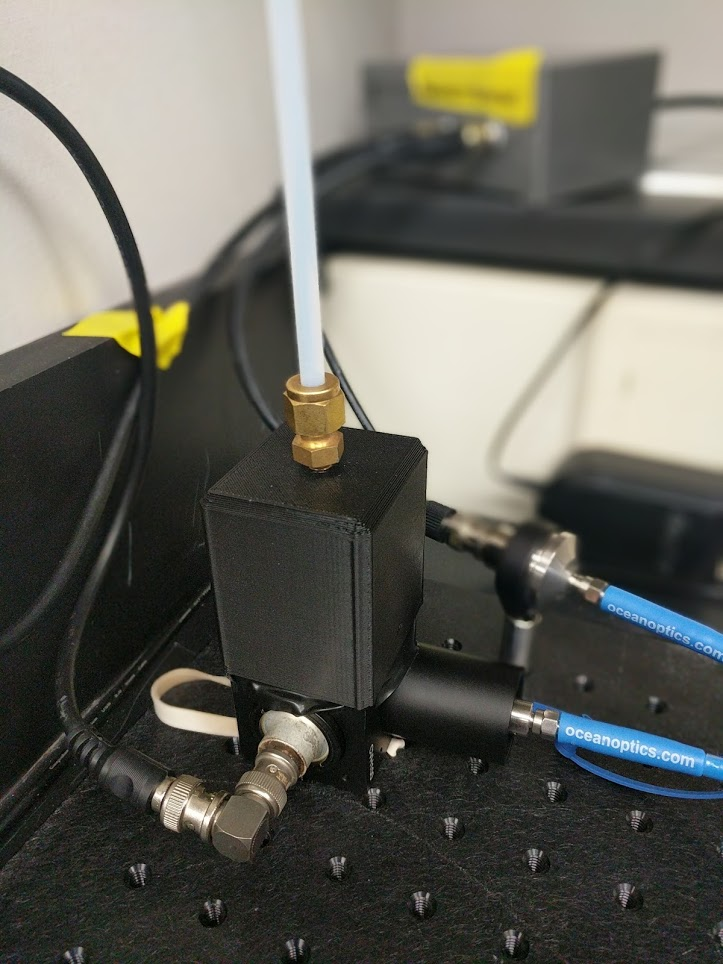
\includegraphics[width=.8\textwidth]{hoye/solutionPL}
\caption{(a) Solution degradation setup for molecular screening with 1. Nitrogen purge line 2. LED intensity measurement 3. Sample chamber 4. LED input 5. PL measurement. (b) Schematic of the sample chamber for solution degradation.  1. Fiber coupled incoming light. 2. Beam Collimator. 3. Dark enclosure with nitrogen purge. 4. Expanded beam covering sample. 5. Cuvette. 6. 3x10 mm solution well. 7. Long pass filter to remove scattered laser light. 8. Photodiode. 9. Light from sample.}
\label{fig:hoye_solutionPL}
\end{figure}

To investigate molecular lifetime, the solution photoluminescence degradation apparatus shown in Figure \ref{fig:hoye_solutionPL} was developed.
This setup uses a 375 nm fiber coupled LED as a pump, powered by a Keithley 26XX source meter.
When operated at the high luminance needed for a pump, UV LEDs suffer from low stability (interestingly, a related problem to the one we are trying to solve).
In order to operate at a constant pump dose during the test and between samples, a feedback loop is implemented using a split fiber.  
This fiber (blue in Figure \ref{fig:hoye_solutionPL}) has two cores, a large 1 mm diameter, as well as a 50 $\mu$m diameter.
The small core is used for the feedback loop to the power supply, adjusting the optical power every 5 minutes during the lifetime.
The large fiber is used to support the high light intensity needed to degrade the sample.


The sample is contained in the black box of Figure \ref{fig:hoye_solutionPL}, which supports a 1 cm by 1cm base dimensioned cuvette.
During this measurement, it is important to evenly degrade the molecules in the solution.
In an unstirred cuvette, it is likely that diffusion of molecules is slower than degradation, so it is important that the excitation condition is evenly applied.
Several steps were implemented to ensure this was true in the testing configuration.
Firstly, as the light passes through the sample, a Beer's law absorption profile creates a difference in the absorbed does between the incident and exiting plane.
Dilute solutions used for this study typically have low absorption, but to minimize this effect, a short light path length is preferred.
This is implemented by using a cuvette with inner dimensions of 10 mm by 3 mm, with the 3 mm to minimize the path length, as shown in Figure \ref{fig:hoye_solutionPL}.
To minimize intensity differences across the face of the cuvette, an expanding beam collimator is used on fiber input.  
This takes the small area fiber input and collimates the beam over a diameter of $\approx$ 1 cm, spreading the beam across the full width of the cuvette.
The beam likely has spatial non-uniformity, but exciting the full width of the cuvette was deemed adequate.
Additionally, the cuvette is only filled partially, to ensure that all of the solution is in the beam.


The tested molecules require highly volatile solvents, so a screw top cuvette is used to minimize evaporation of the solvent.
Emitters are frequently sensitive to oxygen quenching, increasing non-radiative relaxation processes.\supercite{Endo2008,Schueppel2007,Baldo2000}
To avoid this, in addition to the sealed cap with sample preparation in a nitrogen glovebox, the sample chamber is kept under a positive nitrogen pressure using a constant purge, shown as the white plastic line coming into the sample chamber in Figure \ref{fig:hoye_solutionPL}.

\begin{wrapfigure}{r}{.5\textwidth}
\centering
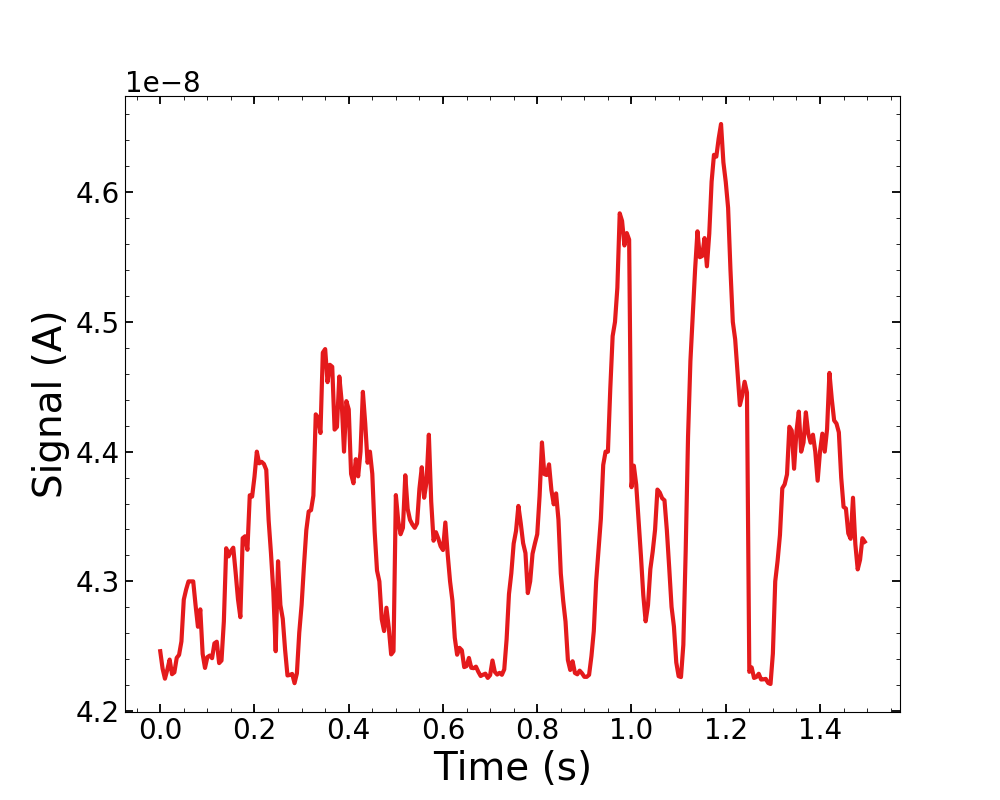
\includegraphics[width=.48\textwidth]{hoye/stir}
\caption{Scatter in signal when stirring.  Despite the noise, notice the constant baseline.}
\label{fig:hoye_stir}
\end{wrapfigure}

Initial tests using this setup showed loss in the photoluminescence that was reversible by physical agitation of the sample.  
This suggested that the molecule is precipitating out of the solution, though no precipitate was visible due to the dilute loading ($10^{-6}$ M).
Because of this, stirring needed to be added to the solution, and was done by adding a spherical stir ball and placing the apparatus on a stir plate.
However, the addition of the stir bar added significant noise to the measured PL signal, shown in Figure \ref{fig:hoye_stir}.
It was found that the movement of the stir bar caused significant scattering of the light and was impacting the measurement.
In addressing this problem, points were taken every 5 ms to observe the scatter.
It was found that a minimum signal was reliably achieved every 300 measurements.
This is believed to be a period where the stir bar is out of the light path and not scattering light.  
To eliminate the noise, 300 points are taken at 5 ms intervals, and the minimum is taken as the solution signal.

This method has been developed and is able to produce reliable results on the same solution.
Test results have started using FIr(pic) as an emitter.
Molecular screening has yet to be done using this technique.

\end{document}
